\section{Hardware-Aware Neural Architecture Search}\label{sec:hw-nas:hwnas}

    \gls{abb:nn} architectures designed through \gls{abb:nas}, while achieving high accuracy and performance, exhibit high complexity and resource-intensive demands, as illustrated in Figure. Consequently, in real-world applications, mere accuracy falls short, given the imperative efficiency constraints imposed by the underlying hardware. Since 2017, a novel wave of \gls{abb:nas} algorithms, known as \gls{abb:hwnas}, has emerged to address this issue. These methods incorporate hardware constraints directly into their objective function and optimize their search space with respect to the target hardware platform.


    In the following section, we will present the latest taxonomy for \gls{abb:hwnas}, as well as the problem formulation and the components of \gls{abb:hwnas} as described by~\cite{hwnas-survey}.

    \subsection{Taxonomy of \gls{abb:hwnas}}
    
        In ~\cite{hwnas-survey}, \gls{abb:hwnas} methods are classified into three categories according to the final hardware target. This subsection presents the taxonomy illustrated in~\Cref{fig:chap1:hw-nas:hwnas} and explains the different categories.

        \begin{figure}[hbt]
            \begin{center}
            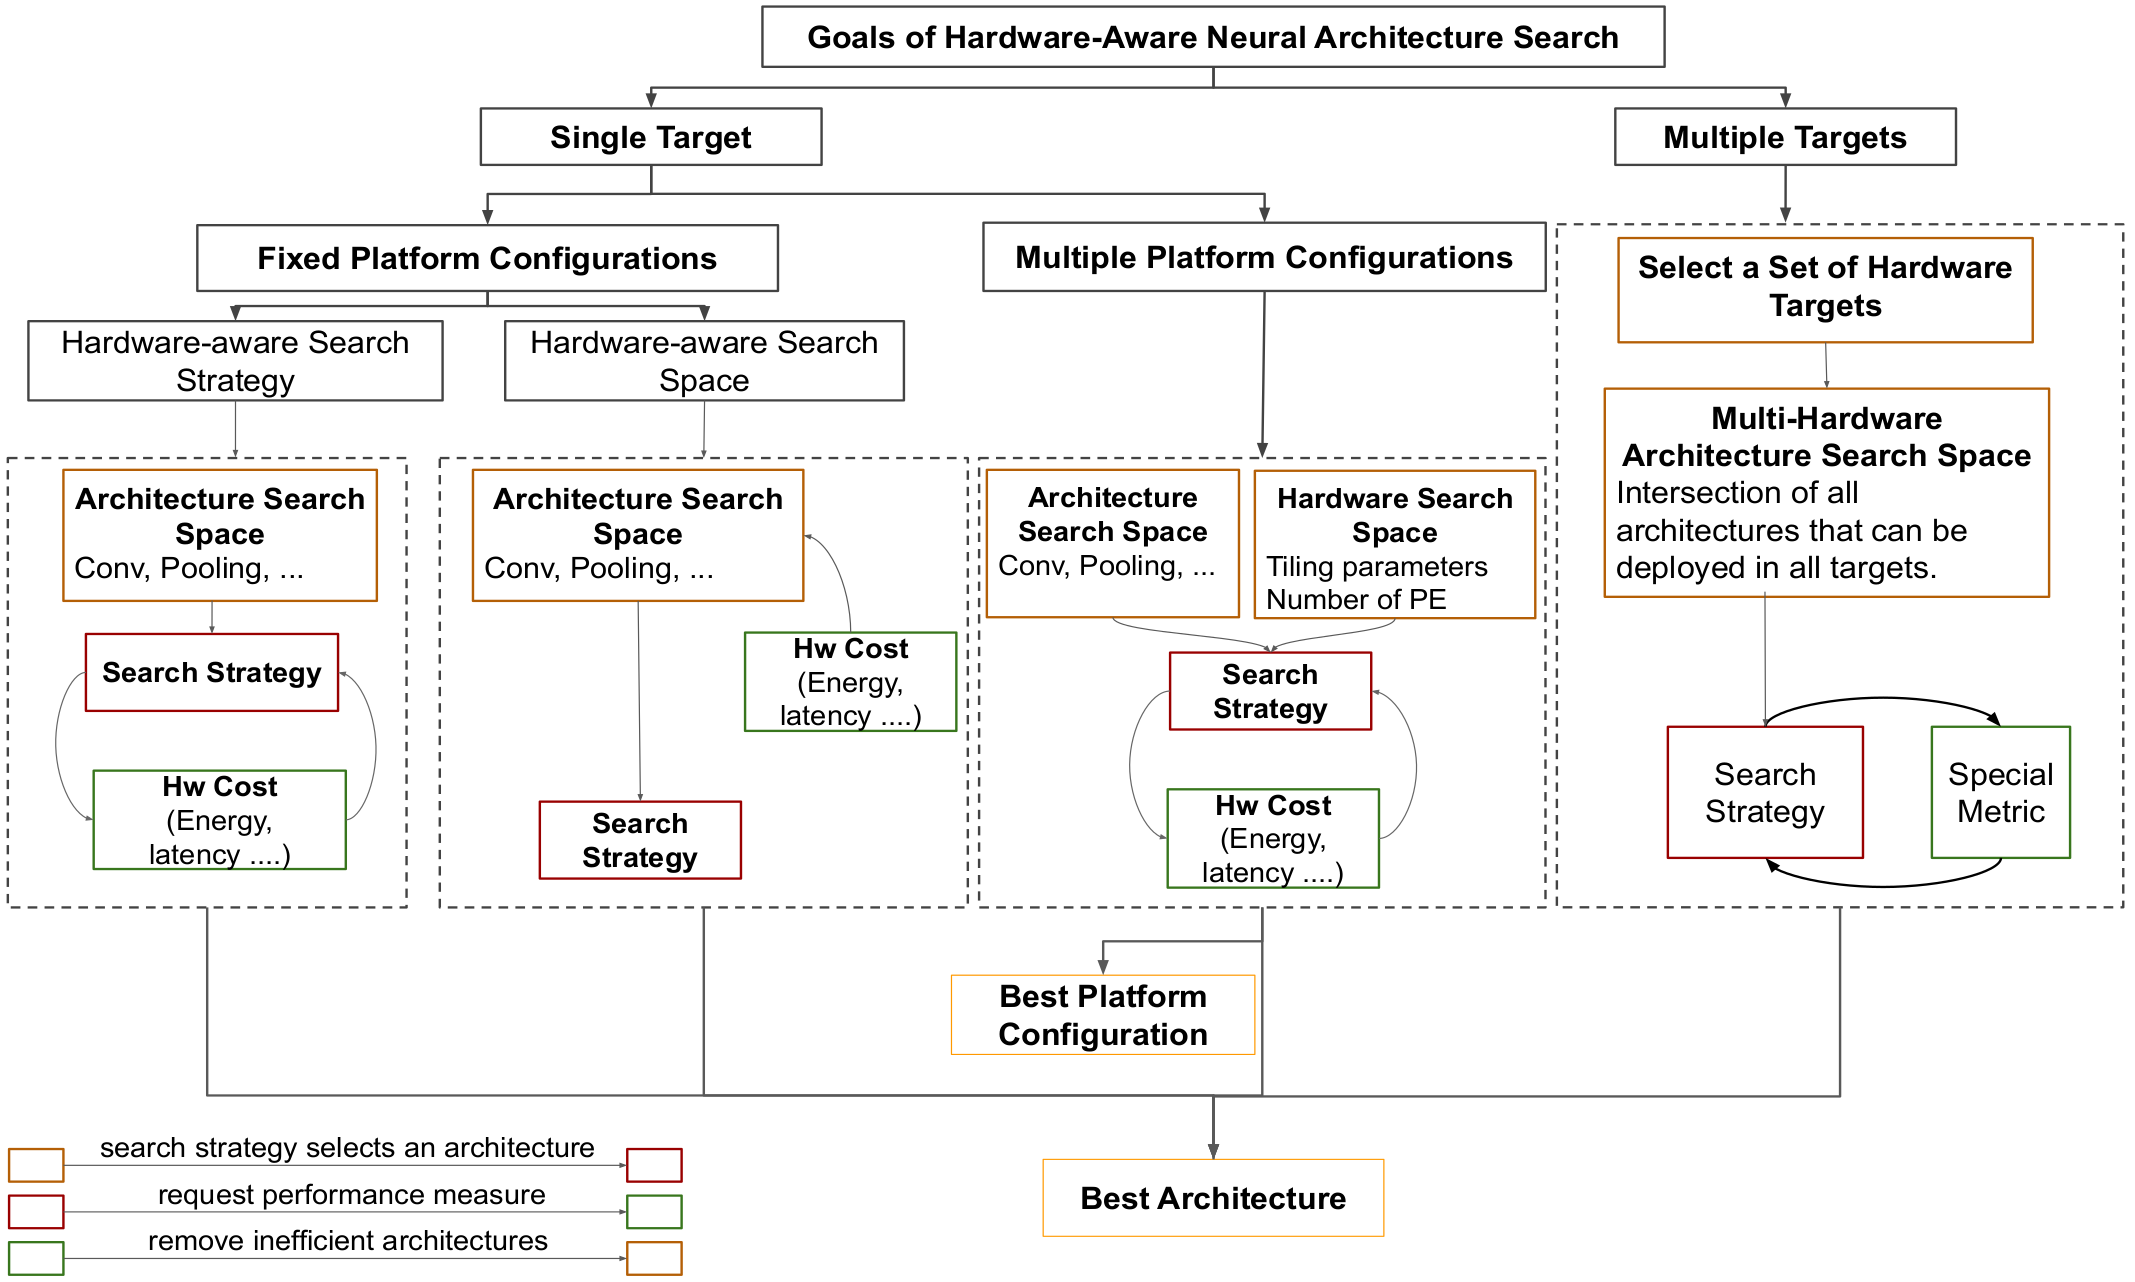
\includegraphics[width=1\textwidth]{assets/images/hwnas-taxonomy.png}
            \end{center}
            \caption{\gls{abb:hwnas} Taxonomy~\cite{hwnas-survey}}%
            \label{fig:chap1:hw-nas:hwnas}
        \end{figure}
        
        Given a target hardware platform and its configurations, the \gls{abb:hwnas} process can be categorized into three main categories : 
        
        \subsubsection{Single Hardware Target with a Fixed Configuration}
            In this category, we have a single hardware platform to target, such as CPU,  GPU, or FPGA,  with only one configuration, given the inherent variability across instances of the same hardware type (e.g. not all CPUs have the same architecture, not all FPGAs have the same specifications). The \gls{abb:hwnas} method will search for the optimal architecture that is optimized for this target hardware with this specific configuration. This objective can be pursued through two distinct approaches:

            \begin{itemize}
                \item The search space is narrowed down to only contain candidates that are compatible with the target platform. This is done by evaluating the performance of operators on the target platform or by defining a set of pruning rules based on prior experimentation. For example, in HURRICANE~\cite{hurricane},  different operator choices are defined for three types of mobile processors: Hexagon DSP, ARM CPU and Myriad Vision Processing Unit (VPU).
                
                \item Alternatively, the search strategy uses a multi-objective problem formulation, considering both accuracy and hardware cost(e.g., latency, memory usage, energy consumption) to guide the search, like in FBNet~\cite{fbnet}. These objectives are measured using different evaluator components.
            \end{itemize}
               

        \subsubsection{Single Hardware Target with Multiple Configurations}
            The \gls{abb:hwnas} methods within this category search for the optimal architecture on multiple configurations of the same target hardware. For example, in the FNAS method~\cite{fnas}, the target hardware is FPGA but the hardware search space includes more than one configuration of this hardware type (e.g., tiling specifications). To streamline the search process, candidate architectures failing to meet the latency constraints associated with these configurations are pruned from the search space.

        
        \subsubsection{Multiple Hardware Targets}
            Within this category, \gls{abb:hwnas} methods search for an architecture that yields high performance across a diverse set of hardware platforms. A notable example of research addressing this challenge is presented by~\cite{multi-target}. The methodology defines a multi-hardware search space, encompassing architectures situated at the intersection of each hardware's individual search space, as illustrated in Figure. The goal of optimizing for a range of hardware architectures is particularly challenging due to the inherent difficulty in finding a model that is well-suited for diverse hardware environments (e.g., CPU and GPU). However, it is the ideal objective to optimize for, especially in applications tailored for mobile devices.

    
    \subsection{Problem Formulations in \gls{abb:hwnas}}
        \gls{abb:hwnas} is an optimization problem that takes different objectives into consideration, namely accuracy and hardware constraints such as latency, memory usage, and energy consumption. The problem formulation is categorized into two distinct optimization classes: single-objective and multi-objective optimization, as outlined in~\cite{hwnas-survey}.
    
        \subsubsection{Single-Objective Optimization}
            Within this class, the optimization problem is approached through two distinct methods:
            \begin{itemize}
                \item Using two-stage optimization, which is sequential optimization process. Initially, the objective to optimize for is accuracy, and then compression techniques are applied to specialize the discovered architecture for the target hardware. For instance, after finding the optimal architecture in terms of accuracy, uses reinforcement learning to select the pruning level and the quantization bitwidth to enhance  the hardware efficiency metrics for the initially discovered architecture.
                \item Using constrained optimization, where the fitness to optimize remains the accuracy, but the optimization process is mathematically contsrained by hardware metrics. Various constrained optimization techniques can be applied to address this problem subclass. As demonstrated in MNASNet, latency is introduced as a learnable penalty term integrated into the fitness function. This ensures that the optimization process not only prioritizes accuracy but also adheres to specified hardware constraints during the search for the optimal architecture.
            \end{itemize}

        \subsubsection{Multi-objective Optimization}
            In this category, the optimization problem can be addressed using two distinct methodologies:
            \begin{itemize}
                \item Using Scalarization Methods, where the multi-objective optimization problem is turned into a single-optimization problem using a weighted aggregation function. This function can be a weighted sum, a weighted exponential sum, a weighted min-max or a weighted product. For example, in~, a weighted sum of the accuracy and energy is used as the objective function to optimize for. 
            \end{itemize}
